% id: 105-20
% book: 100발100중 3-2 중간 · 01 3-2 중간(삼각비·삼각비의 활용·원과 직선·원주각·부록)
% section: 실전 모의고사 3회
% figure: crop:fig-105-20.png
% answer: ②
% answer_source: 답지(빠른정답)
% variant_level: 0 (원본 전사)
% 이 파일은 build.mjs 가 items.json 에서 만든다. 고칠 때는 items.json 을 고친다.
\smash{\raisebox{1.5mm}{\dmkichul{100발100중 3-2 중간 105쪽 20번}}}
\noindent\begin{minipage}[t]{0.58\linewidth}\vspace{0pt}\raggedright 그림과 같이 네 점~$\pt{A}$, $\pt{B}$, $\pt{C}$, $\pt{D}$가 원~$\pt{O}$ 위에 있다. $\arc{AB}:\arc{BC}:\arc{CD}:\arc{DA}=1:2:3:4$일 때, $\angle\pt{BCD}$의 크기는? \mbox{[4점]}\end{minipage}\hfill\begin{minipage}[t]{0.4\linewidth}\vspace{0pt}\centering 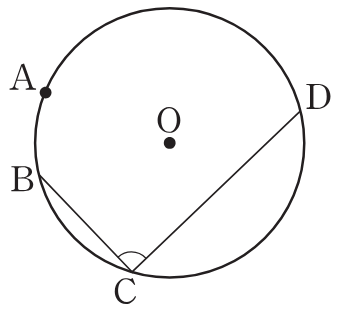
\includegraphics[width=81.5pt]{figures/fig-105-20.png}\end{minipage}\par
\begin{choicesii}{$72^\circ$}{$90^\circ$}{$108^\circ$}{$120^\circ$}{$144^\circ$}\end{choicesii}
